\documentclass[10pt,a4paper,final]{article}
\usepackage[latin1]{inputenc}
\usepackage{amsmath}
\usepackage{amsfonts}
\usepackage{amssymb}
\usepackage{graphicx}
\setlength{\topmargin}{-.5in}
\setlength{\textheight}{9in}
\setlength{\oddsidemargin}{.125in}
\setlength{\textwidth}{6.25in}
\author{Dennis Ideler}
\title{MATH 2P71: Intro to Combinatorics\\Assignment 5: Graph Theory}
\begin{document}
\maketitle

\begin{enumerate}
\item % Q1
Draw all graphs on 5 nodes in which every node has degree at most 2. Assume that graphs are not labelled.
Note: graphs where all nodes have the same degree, are \emph{regular}.

%This is visualized in figure~\ref{q1}.\\

\begin{figure}[h!]
  \centering
    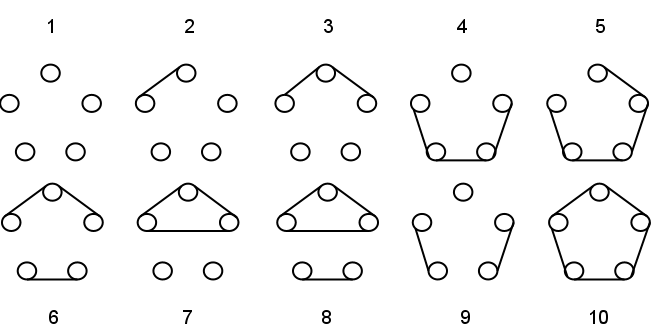
\includegraphics[scale=0.5]{q1.png}
  \caption{10 graphs on 5 nodes in which every node has degree at most 2.}
  \label{q1}
\end{figure}

\item % Q2
How many subgraphs does a 4-cycle have? Assume that the 4-cycles is labelled. \\
\\
The textbook states (as the answer to question 7.2.2) that the edgeless graph on $n$ nodes
has $2^n$ or $\sum_{k=0}^n \binom{n}{k}$ subgraphs, and that a 3-cycle (triangle) graph
has 18 subgraphs. A 4-cycle graph will have $2^4 = 16$ edgeless subgraphs.
We still need to count the subgraphs with edges. \\
\\
\begin{tabular}{|c||c|c|c|c|c|}
\hline 
 & 0 isolated nodes & 1 isolated node & 2 isolated nodes & 3 isolated nodes & 4 isolated nodes \\ 
\hline \hline 
0 edges & 1 & 4 & 6 & 4 & 1 \\ 
\hline 
1 edge &  4 & 8 & 4 & --- & --- \\ 
\hline 
2 edges &  6 & 4 & --- & --- & --- \\ 
\hline 
3 edges &  4 & --- & --- & --- & --- \\ 
\hline 
4 edges &  1 & --- & --- & --- & --- \\ 
\hline 
\end{tabular} 

This can also be written as:

\begin{tabular}{|c||c|c|c|c|c|}
\hline 
 & 0 isolated nodes & 1 isolated node & 2 isolated nodes & 3 isolated nodes & 4 isolated nodes \\ 
\hline \hline 
0 edges & $4 \choose 0$ & $4 \choose 1$ & $4 \choose 2$ & $4 \choose 3$ & $4 \choose 4$ \\ 
\hline 
1 edge &  $4 \choose 1$ & $\binom{4}{1} + \binom{4}{1}$ & $4 \choose 3$ & --- & --- \\ 
\hline 
2 edges &  $4 \choose 2$ & $4 \choose 3$ & --- & --- & --- \\ 
\hline 
3 edges &  $4 \choose 3$ & --- & --- & --- & --- \\ 
\hline 
4 edges &  $4 \choose 4$ & --- & --- & --- & --- \\ 
\hline 
\end{tabular} 

In total, there's 47 subgraphs.

\item % Q3
Let G be a connected graph with at least two vertices. Prove that it has a vertex such that if this vertex is removed (along with all edges incident with it), the remaining graph is connected.\footnote{
The remaining graph can be disconnected, but there is \emph{at least one} vertex that ensures it remains connected.} \\
\\
To find the vertex that we can safely remove:
\begin{enumerate}
  \item Find the longest path\footnote{The longest path problem is the problem of finding a simple path of maximum length in a given graph. A path is called simple if it does not contain any repeated vertices.}
  \item Remove endpoint node of longest path
  \item Graph remains connected
\end{enumerate}

This works because every connected graph contains a spanning tree.\footnote{To get a spanning tree out of a connected graph, remove an edge from any cycle that exists. Continue to do so until the subgraph has no cycles, thus a spanning tree remains.}
Our longest path cannot contain any repeated nodes, so it will be in the form of a spanning tree.
In trees, the endpoint of the longest path will be a leaf node.
As the lemma states, removing a leaf node (our endpoint) produces a tree,
which by definition is connected (a tree is a connected acyclic graph).

\underline{Lemma:} If $T$ is a tree and $n(T) \geq 2$ then $T$ contains at least two leaves.\\
$\therefore$ Deleting a leaf from a tree produces a tree.

\begin{figure}[h!]
  \centering
    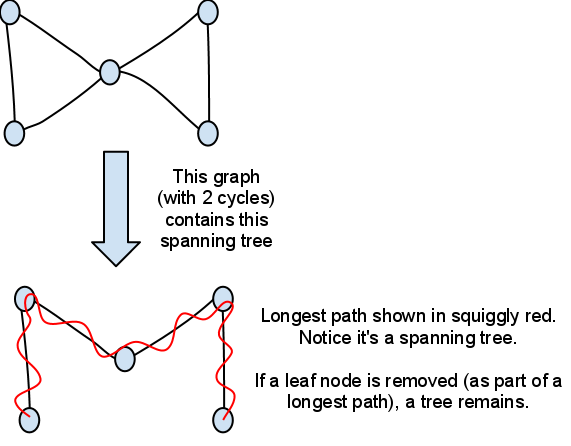
\includegraphics[scale=0.4]{q3.png}
  \caption{Example of how a connected graph with cycles can be reduced to a spanning tree which
  contains the longest path.}
  \label{q3}
\end{figure}

\item % Q4
Does there exists a graph with the following degrees:
\begin{enumerate}
  \item \textbf{0}, 2, 2, 2, 4, 4, \textbf{6} \\
  \\
  No, because there are 7 nodes, and if there exists a node with degree 6,
  it must be adjacent to every other node. Which means there cannot exist a node with degree 0,
  yet one is given.

  \item 2, 2, \textbf{3}, \textbf{3}, 4, 4, \textbf{5} \\
  \\
  No. The Handshaking Lemma states that for any graph $G = (V, E),\: \sum_{v \in V} deg(v) = 2|E|$
which means that the sum of degrees of each of the vertices is equal to the cardinality of the edge-set multiplied by two.

From this we can derive:
\begin{enumerate}
  \item In every graph, the number of nodes with odd degree is even.
  \item No graph of odd order is regular with odd degree.
\end{enumerate}

The first statement says that our graph is impossible because the number of nodes with odd degree is odd (there are 3 of them).  
\end{enumerate}

\item % Q5
Prove that if a tree has a node of degree $d$, then it has at least $d$ leaves. \\
\\
To prove this, we have to find the node in the tree with the highest degree, because
any other node will have a lesser or equal degree and thus cannot have more leaves than the node
with the highest degree. So we find the largest $n$-star which is a subtree.

\begin{figure}[h!]
  \centering
    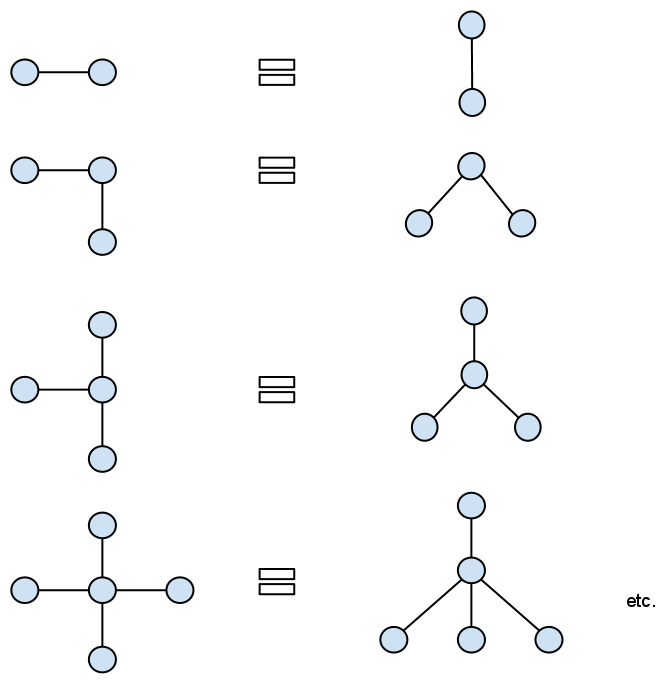
\includegraphics[scale=0.4]{q5.png}
  \caption{$n$-stars are trees (shown here as rooted trees).}
  \label{q5}
\end{figure}

An $n$-star graph has as many leaves as the degree of the centre node (i.e. $n-1$). \\
The tree lemma (mentioned earlier) states that we can remove leaves from the tree and it remains a tree.
So we can do this until we reach the largest $n$-star which is a subtree.
This subtree has a node of degree $d$ (the centre node) and $d$ leaves. So that means the supertree
has at least $d$ leaves since it contains this subtree (and possibly more).

\item % Q6
Take an $n$-cycle, and connect two of its nodes at distance 2 by an edge.
Find the number of spanning trees in this graph. \\
\\
Loosely speaking, a spanning subgraph is a subgraph that contains the same vertex-set as the supergraph,
$V(G') = V(G)$. A spanning tree is a connected acyclic spanning subgraph. \\
\\
To make this problem easier we only consider labelled $n$-cycles.

\begin{figure}[h!]
  \centering
    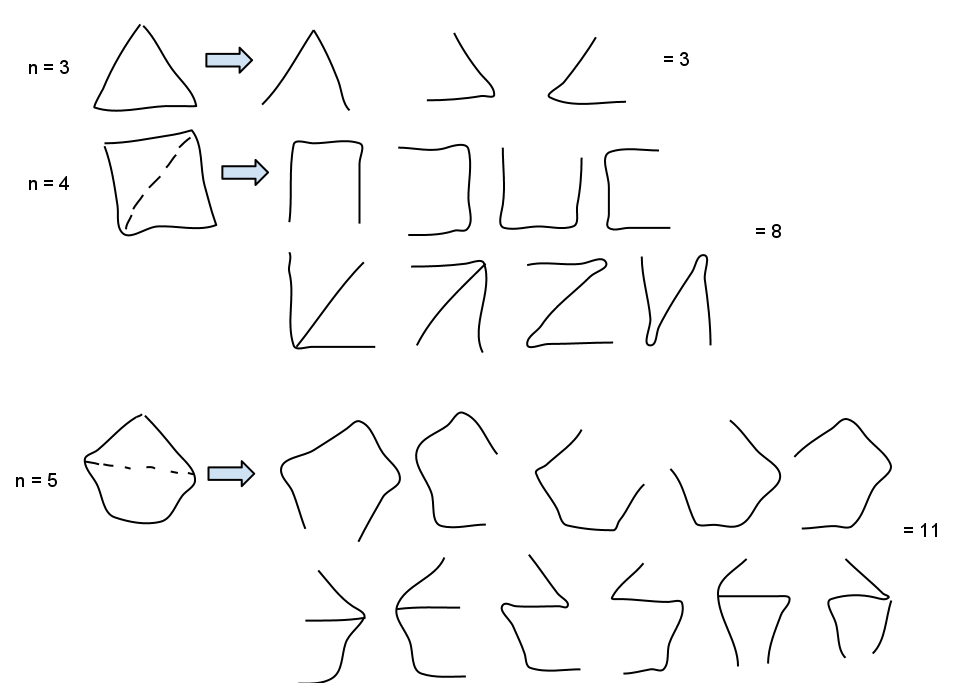
\includegraphics[scale=0.4]{q6.png}
  \caption{Sloppy drawings of all spanning subtrees for $C_3$ to $C_5$.}
  \label{q6}
\end{figure}

Notice a pattern: $C_4 = 4 + \binom{2}{1} + \binom{2}{1} = 8$,
$C_5 = 5 + \binom{3}{2} + \binom{3}{2} = 11$, $C_6 = 6 + \binom{4}{3} + \binom{4}{3} = 14$, etc. \\
There are $n + \binom{n-2}{n-3} + \binom{n-2}{n-3}$ spanning trees in this
modified $n$-cycle graph, except for $n=3$ which has 3 spanning trees.

\end{enumerate}
\end{document}
